\appendix

\section{\label{appendix_1}The reduced equation of motion}

The equation of motion within the context of the Social 
Force Model includes at least six parameters ($m$, $\tau$, $A$, $B$, 
$\kappa$ and $v_d$), but the equation itself barely depends on two. The process 
of parameter's reduction is achieved by defining the (reduced) magnitudes 

\begin{equation}
 \left\{\begin{array}{lll}
         t' & = & t/\tau \\
         r' & =& r/B \\
         v' & = & v/v_d \\
        \end{array}\right.
\end{equation}

The (reduced) equation of motion reads 


\begin{equation}
\displaystyle\frac{d\mathbf{v}'}{dt'}=
\displaystyle\frac{\tau}{m\,v_d}\bigg(\mathbf{f}_d+
\mathbf{f}_s+\mathbf{f}_g\bigg)\label{eqn_appendix_1}
\end{equation}

It is straight forward from Eq.~(\ref{eqn_appendix_1}) that the 
corresponding reduced forces can 
be defined as follows\\

\begin{equation}
 \left\{\begin{array}{lll}
         \mathbf{f}_d' & = & \hat{\mathbf{e}}_d-\mathbf{v}' \\
         && \\
         \mathbf{f}_s' & =& \mathcal{A}\,\exp(r'-d')\,\hat{\mathbf{n}} \\
         && \\
         \mathbf{f}_g' & = & 
\mathcal{K}\,(2r'-d')\,\Theta(2r'-d')\,(\Delta\mathbf{v}'\cdot\hat{\mathbf{t}})\
, 
\hat{\mathbf{t}} \\
        \end{array}\right.\label{eqn_appendix_2}
\end{equation}


\noindent where $\mathcal{A}=A\tau/(m\,v_d)$ and 
$\mathcal{K}=\kappa B\tau/m$. \\ 

Notice that $\mathcal{A}$ and $\mathcal{K}$ are actually the only two 
control parameters in Eq.~(\ref{eqn_appendix_1}) for identical 
pedestrians. The ratio $\tau/m$ is common to both, but the magnitudes 
$Av_d^{-1}$ and $\kappa B$ handle each parameter separately.       \\

The fact that $\mathcal{A}$ and $\mathcal{K}$ share the parameter $\tau$ is 
in agreement with the conclusions outlined in Ref.~\cite{johansson}. The 
relaxation time (or ``net-time headway'') $\tau$ actually ``weights'' the 
effects of the environment on the individual (that is, the social repulsion and 
the friction), and thus, appears as a ``key control parameter'' for the 
fundamental diagram as claimed in Ref.~\cite{johansson}.\\

The role of $\tau$ may be somewhat ambiguous whenever the social 
repulsion becomes negligible with respect to the friction. This may occur if 
some kind of balance exists between neighboring pedestrians in 
symmetrical configurations (\textit{i.e.} in crowded corridors). We may 
hypothesize that the ``key control parameter'' may correspond to either 
$\tau$, or, the friction itself $\kappa$. This is an open question, and a 
first order approach to this matter is outlined in Section~\ref{appendix_2}.\\


\section{\label{appendix_2}A simple model for the corridor}

A toy model for a moving crowd along a corridor is the one represented 
schematically in Fig.~\ref{pasillo}. Pedestrians (circles in 
Fig.~\ref{pasillo}) 
are assumed to be lined up from side to side across the corridor, at any given 
position. Social forces in the $x$-direction are further considered to vanish 
because of translational symmetry. Thus, only the sliding friction is allowed 
to balance the the pedestrians own desire. The (reduced) movement equation for 
the $x$-direction according to Section~\ref{appendix_1} and Fig.~\ref{pasillo} 
is  \\

\begin{figure}[htbp!]
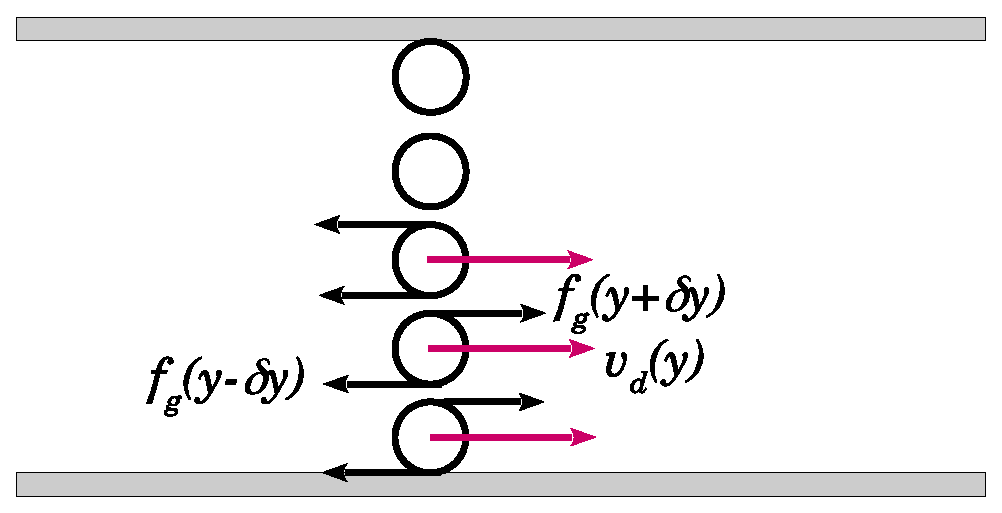
\includegraphics[width=\columnwidth]
{./plots/pasillo.eps}
\caption{\label{pasillo} Schematic diagram for individuals in a corridor. 
The circles represent pedestrians moving from left to right. The desired force 
(red arrows) and sliding friction (black arrows) are assumed to be the only 
relevant forces.}
\end{figure}

 
\begin{equation}
\displaystyle\frac{dv'}{dt'}(y')=1-v'(y')+f_g'(y'+\delta 
y')-f_g'(y'-\delta y')\label{eqn_appendix_2:1}
 \end{equation}

where $v'(y')$ corresponds to the (reduced) velocity (for the $x$-direction) of 
the individual located at the $y'$ position. Notice that the individuals 
remain at the same $y'$ position while traveling through the corridor, since 
balance is expected to take place across the corridor. These positions are 
roughly $\delta y'$, $3.\delta y'$, $5.\delta y'$,.... Actually, it is not 
relevant (for now) the value of $y'$, and a further simplification can be done 
by labeling $v'(y')=v_i$ and $v'(y'\pm 2.\delta y')=v_{i\pm 1}$. The velocity 
of the individual in contact with the bottom wall in Fig.~\ref{pasillo} will be 
labeled as $v_1$. \\  

The last two terms in Eq.~(\ref{eqn_appendix_2:1}) correspond to the 
net drag applied on the pedestrian with velocity $v_i$. According to 
Eq.~(\ref{eqn_appendix_2}) this drag may be expressed as

\begin{equation}
 f_{g,i+\frac{1}{2}}'-f_{g,i-\frac{1}{2}}'=
  \left\{\begin{array}{lcl}
          2\alpha\,v_{2}-3\alpha\,v_{1} &  & i=1 \\
          & & \\
          2\alpha\,(v_{i+1}-2v_i+v_{i-1}) & & i>1\\
         \end{array}\right.\label{eqn_appendix_2:2}
\end{equation}

\noindent for $\alpha=\mathcal{K}(r'-\delta y')$. Recall that our first order 
approach considers $\delta y'$ as roughly uniform across the corridor.  \\

The stationary situation can be computed straight forward from 
Eq.~(\ref{eqn_appendix_2:1}). Thus, for $\dot{v}_{i}=0$ the following set of 
equations determine the velocity profile in the corridor (within this toy 
model)

\begin{equation}
  \left\{\begin{array}{lcl}
          (3\alpha+1)\,v_{1} - 2\alpha\,v_{2} & = & 1 \\
          & & \\
          -2\alpha\,v_{i-1}+(4\alpha+1)\,v_i-2\alpha\,v_{i+1} & = & 1\\
         \end{array}\right.\label{eqn_appendix_2:3}
\end{equation}

Notice from  Eq.~(\ref{eqn_appendix_2:2}) that $\alpha=0$ means no friction at 
all, and thus, the individuals are allowed to move free from drag. It can be 
verified that $v_i=1$ solves the set (\ref{eqn_appendix_2:3}) for this 
scenario. The $\alpha=0$ scenario is expected to occur, however, for densities 
below a contacting threshold.  \\

A boundary condition needs to be imposed in order to solve 
Eqs.~(\ref{eqn_appendix_2:3}) for $\alpha\neq 0$. We fix 
$v_i=v_{i+1}$ at the middle of the corridor since the velocity profile 
should be specularly distributed with respect to the mid-axis of the 
corridor. Fig.~\ref{fig:appendix_2:1} shows the computed mean velocity for the 
bottom side profile as function of $\alpha$.\\


\begin{figure}[htbp!]
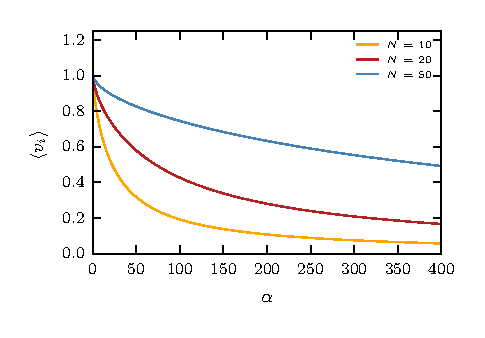
\includegraphics[width=\columnwidth]
{./plots/fig_velocity_model.eps}
\caption{\label{fig:appendix_2:1} Mean velocity of the bottom half of the 
individuals vs. the parameter $\alpha$. Both axis are dimensionless. $N$ 
corresponds to the number of individuals. }
\end{figure}

Fig.~\ref{fig:appendix_2:1} exhibits a decreasing behavior for increasing 
values 
of $\alpha$. As explained above, the maximum value occurs at $\alpha=0$ 
(\textit{i.e.} $\langle v_i\rangle=1$). However, the decreasing slope slows 
down for increasing number of individuals. This corresponds to a flattening in 
the velocity profile, (see Section\ref{results} for details).  \\   

The mean flux of individuals can be built from the mean velocity and the 
corresponding pedestrian density as follows

\begin{equation}
 J=\left\{\begin{array}{lcl}
          \rho & \mathrm{for} & \alpha=0 \\
          & & \\
          (\rho_0+c\,\alpha)\,\langle v_i\rangle & \mathrm{for}  & 
\alpha>0\\
         \end{array}\right.\label{eqn_appendix_2:4}
\end{equation}

where $\langle v_i\rangle$ equals unity for the case $\alpha=0$, and thus, it 
was omitted in (\ref{eqn_appendix_2:4}). The density $\rho=\rho_0+c\,\alpha$ 
corresponds to the packing density (that, the density above the contacting 
threshold) and $c$ corresponds to a somewhat ``packing coefficient''. 
Fig.~(\ref{fig:appendix_2:2}) shows the flux as a function of the density, 
assuming $\rho_0=1$ for simplicity. \\


\begin{figure}[htbp!]
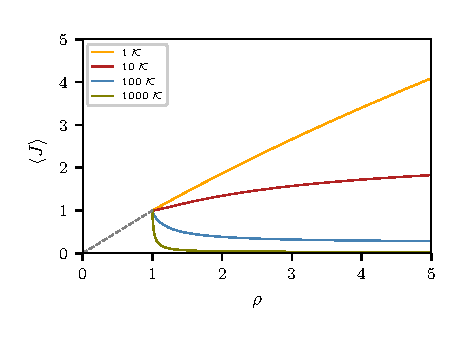
\includegraphics[width=\columnwidth]
{./plots/fig_flux_model.eps}
\caption{\label{fig:appendix_2:2} Mean flux of the bottom half of the 
individuals vs. the pedestrian (global) density $\rho$ (see text for 
details). Both axis are dimensionless. The number of individuals across the 
corridor was set to $N=10$, and the contacting threshold was set to $\rho_0=1$. 
The dashed line corresponds to the flux at the low density regime (say, 
$\langle 
v_i\rangle=1$.   }
\end{figure}


The pedestrian flux $J$ attains two possible behaviors, according to 
Fig.~\ref{fig:appendix_2:2}. For packing coefficients $c<0.05$, the flux 
diminishes as the corridor becomes more crowded. But, if $c$ surpasses this 
threshold, the flux slope becomes positive, although the mean velocity 
diminishes. We conclude that the role of the pedestrians' density is crucial 
for building the fundamental diagram.   \\
